\documentclass[12pt]{article}
\usepackage{amsmath}
\usepackage[english]{babel}
\usepackage{graphicx}
\usepackage{verbatim}
\usepackage{wrapfig}
\usepackage{float}
\usepackage[top=1in, bottom=1in, left=1in, right=1in]{geometry}
%\usepackage{times}
\usepackage{hyperref}
\hyphenpenalty=5000
\tolerance=1000
\setlength\parindent{0pt}
\begin{document}
\title{Network Simulation}
\author{Maxwell Horton, Alex Jose, Michael Lauria, Anish Agarwal, Johno Ikpeazu}


\maketitle
\noindent
\tableofcontents
\newpage
\section{Introduction}

\begin{figure}[t]
\centering 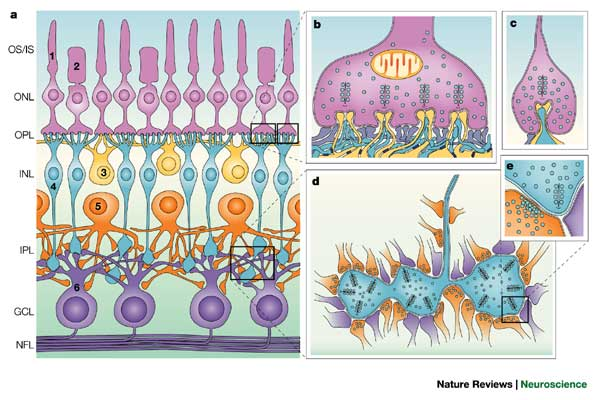
\includegraphics[scale=1.]{figures/cells_2.jpg}
\caption{Examples of cells of the retina.}
\label{fig:test}
\end{figure}

\section{Simulation Architecture}


\subsection{Event-Driven Simulation}
An event-based simulation was used. All network objects (hosts, links, routers and flows) were children of the same parent class named event-generators. Every event-generator had its own priority queue that it could throw events on. The ordering of the priority queue was by the timestamp of the events that each event-generator generated. There was a global handler that checked the minimum timestamp of each network object in each loop and processed the event with the smallest overall timestamp in the simulation in the loop. Processing an event essentially means giving that event to the destination specified in the event itself (the source and destination of events have to necessarily be adjacent in the network topology or the source and destination must be the same). 

Provided below is a high level description of what happens in each simulation loop:
\begin{enumerate}
\item Global handler iterates over Event Generators
\item Generators report their internal event queues (\emph{events are deterministic -> know when they should trigger})
\item Simulator collects set of most-immediate events and sends them to their respective destination
\item Generators that have been given events react and generate new events with a later timestamp that they push onto their respective priority queues
\end{enumerate}

\subsection*{Reflection on event-based simulation}
The event-driven simulation paradigm ended up working well for our group. While it may initially be less intuitive than a continuous simulation, and plotting was sometimes difficult (as data is typically only logged for times where interesting things are happening), an event-based simulation is particularly well-suited for simulating networks, and was fairly simple to implement.


\subsection{Links}

Links are bi-directional with each side of a link having the same buffer-size and capacity. Links keep adding packets to their buffer until it has reached its maximum buffer occupancy, at which point it drops all subsequent packets until its buffer occupancy has dropped below the maximum. This is a short description of the procedure the link utilizes to update its link size and capacity:

\begin{enumerate}
\item Link gets an event – finds the difference between the packet event and its own internal clock
\item Decreases buffer occupancy by the difference in time multiplied by capacity
\item If buffer occupancy + packet size is smaller than max buffer occupancy, add packet to its buffer
\item Update queue delay, buffer size and internal clock (based on event time)
\item Add an event to its priority queue that essentially tells the handler to send the packet to the adjacent network object at the appropriate time
\item (event time + propagation delay + queue delay)
\end{enumerate}

\subsection*{Reflection on Links}

Links were relatively straightforward to write. A conceptual error we made at the start was that we gave a link a single buffer, which had packets added to it simultaneously from both sides of the link. We managed to rectify this error relatively quickly. Logging was particularly difficult for links as we had to estimate the instantaneous link rate for a link based only on the information we get when a link receives an event. This procedure has been described in the segment of the report dealing with plotting. 





\subsection{Routers}

Routers run a distributed bellman-ford algorithm to find the shortest path between any pair of hosts. Each router has a routing table that is uses to figure out which neighboring link it should send information down for each flow. The routing table is implemented as an unordered map with the key being the host ID and the value a path from that router to that host.
 
A path is a vector of 3-tuples. The elements on the 3-tuple are the link ID, the delay on that link, and the most recent time the router updated the delay for that specific link. So a path from router to a host gives the exact set of links that will be traversed to get to that host and the total delay to that host.
 
At specified time intervals, a router will broadcast its routing table to all adjacent routers. Before broadcasting its table, it will find the most recent link delay for every neighboring links and update each path it has with the correct delay and update time. The time a router waits between broadcasting its routing table is given by the following formula: 
% make this mathy!
$$waitTime = min(5.0, waitTime + 0.1)$$

When a router receives a routing table from a neighboring router, it first updates all the relevant link weights in every path that it has if the link update time in the neighbor router’s, routing table is more recent.

It then executes the following procedure to check whether it should update the shortest path it has to each host. For each host in neighbors routing table, it checks if two conditions are met:
\begin{enumerate}
\item (Link delay between two hosts ink delay between two hosts + Total delay on other router’s path to host) < current distance of router to host
\item The path between the specified host and the neighbors router and current router do not form a cycle
\end{enumerate}
If both conditions are met, then it updates its routing table with the neighboring router’s path to that host (and appending the link between the two routers to that path).


\subsection*{Reflection on routers}
 
The main challenge we faced with routers was that old routing tables were being bounced around the network. The reason for this was that routers were initially not checking to see how old the routing table information they were getting was. Hence a router did not have an accurate estimation for what the actual link delay on a link was. The change we made to rectify this was that each link in a path was a given a most recent update time attribute. This allowed us to easily enforce that each link delay in a path in a router was only updated if information it received was recent enough. An assumption made with routers is that there is no delay between them receiving a data packet and sending it down the correct link



\subsection{Host}
The host receives PacketEvents from the handler through its giveEvent() function.  This function is split into several cases that are handled by helper functions.  The most common case is that a PacketEvent is received by the host.  In this case, the host is either at the sending or the receiving end of the flow.  To determine this, the host has two maps: ``flows'' and ``recvd''.  The former associates flow ids with the Flow objects whose sending ends are rooted at the host.  The latter associates flow ids with a list of received packets.  Since flow ids must be globally unique, we can determine whether a the host is at the sending end or receiving end of the flow with which the packet is associated.  (We can also use the information on whether the packet is an ack to do this).
\\\\
When a data packet is received, if it is an ACK, the host performs the appropriate action using the ``recvd'' object.  If it is not an ACK, the host passes the event to the appropriate Flow in ``flows'' using the flow id field of the packet.  Non-data packets (i.e. SYNs and FINs) are handled separately.

\subsection{Flow}
The Flow object handles many of the basic operations generic to Vegas and Tahoe.  It contains methods for opening connections, sending packets / adjusting window sizes, etc.

\subsection{VegasFlow}
Our implementation of Vegas updates on a timer set to fire once every RTT.  To do so, a VegasUpdateEvent is generated when the Flow connection is opened (i.e. when the SYNACK is received).  When the VegasUpdateEvent reaches the Host on which the VegasFlow object lives, it is passed to the VegasFlow to be handled.  To handle the VegasUpdateEvent, the window size is adjusted according to:
$$ w(t + 1) = \begin{cases} w + 1, & \gamma < \alpha / minRTT \\ w, & alpha \le \gamma \le \beta \\ w - 1, & \beta < \gamma \end{cases}, \gamma = \dfrac{w}{minRTT} - \dfrac{w}{RTT} $$,
\\\\
where RTT is the most recent RTT.

\subsection{TahoeFlow}
The Tahoe flow resets to slow start on receipt of three duplicate acks, or on a timeout.  If a such a reset occurs, the time of the reset is stored.  Any potential timeouts that would be triggered by an event generated before this time are ignored (to prevent the algorithm from being bombarded by timeouts).  Similarly, we ignore the duplicity of acks for packets with timestamps from before our most recent reset (because otherwise, the algorithm would be bombarded by a barrage of resets).  During slow start, the window size increases by one with every ack until the ssthresh is met.  In congestion avoidance, window size increases by $1/w$ with every ack.

\subsection{Input}
1) Input

Network description files consist of plain-text listings of various network components and their initialization parameters. Flex and Bison were used to lex and parse the network description files. Strings and floating-point numbers can be used to provide arguments, and references to previously-made objects can be made as well. For example, the description file for test case 1 is as follows:
\begin{verbatim}
# Network spec for test case 1
# link stuff link_rate stuff side1 side2 name
link 524288 0.01 12500000 host1   router1 link0
link 524288 0.01 10000000 router1 router2 link1
link 524288 0.01 10000000 router1 router3 link2
link 524288 0.01 10000000 router2 router4 link3
link 524288 0.01 10000000 router3 router4 link4
link 524288 0.01 12500000 router4 host2   link5
# host host_link name
host link0 host1
host link5 host2
# router [list of hosts] [adjacent links] name
router [host1 host2] [link0 link1 link2] router1
router [host1 host2] [link1 link3]       router2
router [host1 host2] [link2 link4]       router3
router [host1 host2] [link3 link4 link5] router4
# flowtype name destination stuff origin window_size stat_time
vegas flow1 host2 160000000 host1 1 0.5
\end{verbatim}

\subsection*{Reflection on Input}

After we settled on a simple format for the network description files, writing the lexer and parser were not too difficult due to the power of flex and bison. There were some strange issues with lexed strings overwriting each other when being accessed in the parser, but all of this was handled by using a string buffer to avoid depending on flex successfully preserving the value of multiple strings.



\subsection{Output}

Network output is logged by each network object through calls to a logging library. Each call to the logger is ‘self-documenting’ in the sense that the calling network object can pass its own label to the logger such that the logger can appropriately tag the passed data for easier plotting at a later point in time.

Plotting is accomplished using Gnuplot-iostream, which allows for plotting with Gnuplot in C++ through simply writing data to the standard output stream.

\subsection*{Reflection on Output}
One significant annoyance with the output code stemmed from the event-based nature of our simulation - it’s simple to get logging data from network objects when they’re sending or receiving events, but getting them to log data when no events are being passed is relatively more difficult. This is not a major problem, as interesting things are happening primarily when events are being passed, but was still a slight problem.


\section{Analysis}
\subsection{Test Case 0}
\subsection{Test Case 1}
\subsection{Test Case 2}
\section{Difficulties}
\appendix
\section{Instructions on Compiling and Input}

\end{document}
